\documentclass[a4paper,13pt]{scrartcl}
\usepackage[left=2.5cm, right=4.5cm, top=2.5cm, bottom=2cm]{geometry}
\usepackage[ansinew]{inputenc}
\usepackage{ngerman}
\usepackage{bibgerm}
\usepackage[T1]{fontenc}
\usepackage{amsmath}
\usepackage[linguistics]{forest}
\usepackage{pict2e}
\usepackage{tikz}
\usepackage{textcomp}
\usetikzlibrary{shapes,arrows}
\setlength\parindent{0pt}

\tikzset{%
  block/.style    = {draw, thick, rectangle, minimum height = 3em,
    minimum width = 3em},
  sum/.style      = {draw, circle, node distance = 1.5cm}, % Adder
  input/.style    = {coordinate}, % Input
  output/.style   = {coordinate}, % Output
   base/.style = {rectangle, rounded corners, draw=black, minimum width=2cm, minimum height=1cm, text centered}
}

\title{test test}
\author{Philipp Bleimund}
\date{15.07.2021}

\begin{document}

\maketitle
\tableofcontents

\section{Threads und Prozesse}

Prozesse sind die ausfuehrung eines Programms auf dem Prozessor.
Jedoch kann ein Prozessor maximal ein Prozess gleichzeitig ausf�hren. Um verwirrung zu beseitigen moechte ich darauf hinweisen, dass selbst moderne
Prozessoren nicht in der Lage sind mehrere Prozesse auszuf�hren. Diese "Ilusion wird erzeugt, da ein Prozessor(Bauteil) mehre Kerne hat. Diese Kerne sind die eigentlichen Prozessoren.
In Zukunft werde ich den Begriff Kerne nutzen um die Unterscheidung zu erleichtern.
Um trotzdem mehrere Prozesse gleichzeitig zu bearbeiten, werden den einzelnen Kernen die Prozesse f�r nur wenige millisekunden zugeordnet.

\subsection{Aufbau von Prozessen}

\begin{center}
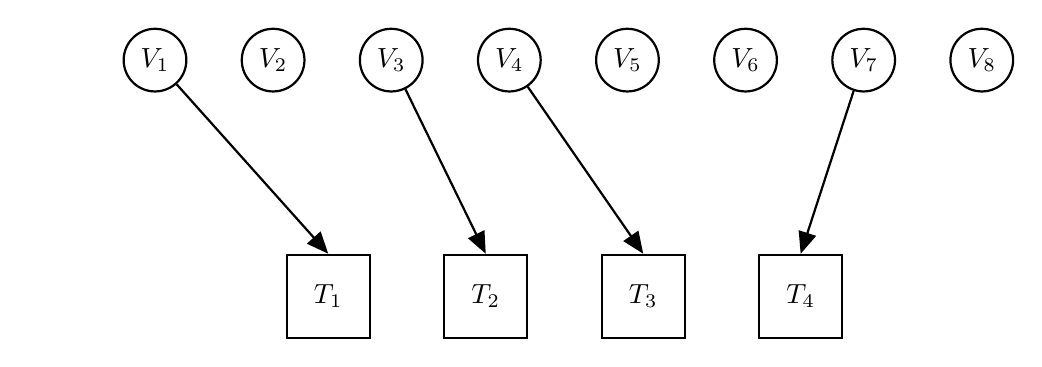
\begin{tikzpicture}[auto, thick, node distance=2cm, >=triangle 45]
\draw
	node at(0,0)[name=start1]{}
	node [sum, name=VThread1, right of=start1]{$V_1$}
	node [sum, name=VThread2, right of=VThread1]{$V_2$}
	node [sum, name=VThread3, right of=VThread2]{$V_3$}
	node [sum, name=VThread4, right of=VThread3]{$V_4$}
	node [sum, name=VThread5, right of=VThread4]{$V_5$}
	node [sum, name=VThread6, right of=VThread5]{$V_6$}
	node [sum, name=VThread7, right of=VThread6]{$V_7$}
	node [sum, name=VThread8, right of=VThread7]{$V_8$};
\draw
	node at(1.7,-3)[name=start2]{}
	node [block, name=Thread1, right of=start2]{$T_1$}
	node [block, name=Thread2, right of=Thread1]{$T_2$}
	node [block, name=Thread3, right of=Thread2]{$T_3$}
	node [block, name=Thread4, right of=Thread3]{$T_4$};
	\draw[->](VThread1) -- node{} (Thread1.north);
	\draw[->](VThread3) -- node{} (Thread2.north);
	\draw[->](VThread4) -- node{} (Thread3.north);
	\draw[->](VThread7) -- node{} (Thread4.north);
\end{tikzpicture}
\end{center}

\subsection{Aufbau von Prozessen}

Prozesse müssen jedoch noch ein wenig mehr als nur ein Stück code besitzen, um aktiv zu werden. Generel kann man sagen, dass Prozesse aus 7 Elementen bestehen.
Diese nennt man Prozesskontext. Innerhalb des Prozesskontextes gibt es noch den Hardwarekontext.
\begin{itemize}
\setlength\itemsep{0.5mm}
\item Das auszuführende Programm
\item Die Daten des Programmes. Umfasst etwa die Globalen variablen.
\item Einen Stack. Ein Stack funktioniert nach dem push und pop verfahren und speichert die lokalen Variablen f�r einen schnelleren zugriff.
\item Zugriffsrechte Des Programmes.
\item Kernelstack. Umfasst die Systemaufrufe des Prozesses.
\begin{itemize}
\item CPU Register. Kann in den meisten F�llen nur ein Befehl speichern (64bit Prozessor = 64bits im Register)
\item MMU Register, dass den zugriff auf den Arbeitsspeicher verwaltet.
\end{itemize}
\end{itemize}

\subsection{Leben eines Prozesses}
\begin{center}
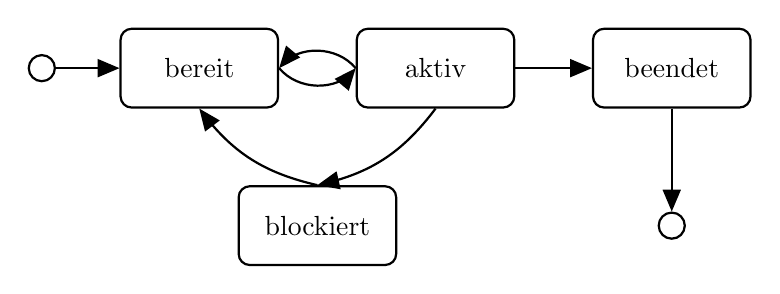
\begin{tikzpicture}[auto, thick, node distance=2cm, >=triangle 45]
\draw
	node at(0,0)[sum, name=start]{}
	node [base, name=bereit, right of=start]{bereit}
	node [base, name=aktiv, node distance=3cm, right of=bereit]{aktiv}
	node [base, name=beendet, node distance=3cm, right of=aktiv]{beendet};
\draw
	node at(3.5,-2)[base, name=blockiert]{blockiert}
	node [sum, name=friedhof, node distance=2cm, below of=beendet]{};
\draw[->](start) -- node{} (bereit.west);
\path[->](bereit.east) edge[bend right=50] node{} (aktiv.west);
\path[->](aktiv.west) edge[bend right=50] node{} (bereit.east);
\path[->](aktiv.south) edge[bend left=20] node{} (blockiert.north);
\path[->](blockiert.north) edge[bend left=20] node{} (bereit.south);
\draw[->](aktiv.east) -- node{} (beendet.west);
\draw[->](beendet.south) -- node{} (friedhof);
\end{tikzpicture}
\end{center}

\subsection{In Windows}
\subsection{Auf der CPU}
\subsection{Implementation in java}
\subsubsection{ThreadPool}
\subsubsection{Thread sicherheit}

\section{Quellen}
MapBild : 
SynchronousJFXFileChooser : https://stackoverflow.com/questions/28920758/javafx-filechooser-in-swing
Answer from Sergei Tachenov
\end{document}